\documentclass{standalone}
\usepackage{tikz}
\usetikzlibrary{external}
\tikzexternalize[prefix=tikz/]

%═══════════════════════════════════════════
% Math packages
%═══════════════════════════════════════════
\usepackage{amssymb,amsthm,amsmath}
\usepackage{mathtools}
\usepackage{proof}
\usepackage{bussproofs}
\usepackage{marvosym}

%═══════════════════════════════════════════
% Environments
%═══════════════════════════════════════════
\theoremstyle{definition}
\newtheorem{definition}{Definition}
\newtheorem{theorem}{Theorem}
\newtheorem{lemma}[theorem]{Lemma}
\newtheorem{claim}{Claim}
\newtheorem{corollary}{Corollary}
\newtheorem{proposition}{Proposition}
\newtheorem{example}{Example}
\newtheorem{remark}[theorem]{Remark}
\newenvironment{sketch}{\begin{proof}[Proof Sketch]}{\end{proof}}

%═══════════════════════════════════════════
% Graphics packages
%═══════════════════════════════════════════
\usepackage{tikz}
\usepackage{graphicx,adjustbox}
\usetikzlibrary{positioning,calc,arrows.meta,shapes.geometric,fit, backgrounds}

% Colors
\definecolor{gruvwhite}{HTML}{f9f5d7}
\definecolor{gruvgreen}{HTML}{79740e}
\definecolor{gruvblue}{HTML}{076678}
\definecolor{gruvpurple}{HTML}{8f3f71}
\definecolor{gruvyellow}{HTML}{d79921} % b57614
\definecolor{gruvred}{HTML}{9d0006}
\definecolor{gruvblack}{HTML}{3c3836}
\definecolor{gruvgrey}{HTML}{7c6f64} %7c6f64

% Colors
\colorlet{backgroundcolor}{gruvblack}
\colorlet{blockbodybgcolor}{gruvwhite}
\colorlet{blockbodyfgcolor}{black}
\colorlet{blocktitlefgcolor}{gruvwhite}
\colorlet{blocktitlebgcolor}{gruvred} % default, but changeable
\colorlet{framecolor}{gruvred}
\colorlet{titlefgcolor}{black}
\colorlet{titlebgcolor}{gruvwhite}


\colorlet{notebgcolor}{gruvblue}
\colorlet{notefgcolor}{gruvgreen}
\colorlet{noteframecolor}{gruvred}

%═══════════════════════════════════════════
% Custom Commands, General Use
%═══════════════════════════════════════════
\newcommand{\key}[1]{\emph{#1}}
\newcommand{\Rat}{\mathbb{Q}}
\newcommand{\Nat}{\mathbb{N}}
\newcommand{\State}{\mathsf{State}} 
\newcommand{\semantics}[1]{[\![\mbox{\em $ #1 $\/}]\!]}
\newcommand{\Model}{\mathcal{M}}
\newcommand{\Nodel}{\mathcal{N}}
\newcommand{\lang}{\mathcal{L}}
\newcommand{\uplang}{\mathcal{L}^\ast}
\newcommand{\vocab}{\mathcal{V}}
\newcommand{\wocab}{\mathcal{W}}
\newcommand{\set}[1]{\{ #1 \}}
\newcommand{\proves}{\vdash}
\renewcommand{\o}{\cdot}
\newcommand{\orr}{\vee}
\newcommand{\andd}{\wedge}
\newcommand{\nott}{\neg}
\newcommand{\bigandd}{\bigwedge}
\newcommand{\quadiff}{\quad \mbox{ iff } \quad}
\newcommand{\rem}[1]{\relax}
 \newcommand{\NP}{\mbox{\sc np}}
\newcommand{\axiom}{\textsc}
\newcommand*{\bigchi}{\mbox{\Large$\chi$}}% big chi
\newcommand{\degree}[1]{\mathrm{deg}(#1)}
\newcommand{\preds}[1]{\mbox{preds}(#1)}
\newcommand{\layer}[1]{\mathsf{layer}(#1)}
\newcommand{\activ}[2]{\mathsf{activ}_{#1}(#2)}
\newcommand{\layerNoArgs}{\mathsf{layer}}

\newcommand{\negweightscore}[1]{\mathsf{nws}(#1)}
\newcommand{\minscore}{\mathsf{mnws}}
\newcommand{\numiterations}{\mathsf{iter}}

%═══════════════════════════════════════════
% Custom Commands, Hebbian Learning
%═══════════════════════════════════════════
\newcommand{\AllNets}{\mathsf{Net}}
\newcommand{\Net}{\mathcal{N}}
\newcommand{\op}{\mathsf{op}}
\newcommand{\Prop}{\mathsf{Prop}}
\newcommand{\Reach}{\mathsf{Reach}}
\newcommand{\Hebb}[2]{\mathsf{Hebb}(#1, #2)}
\newcommand{\HebbNoArgs}{\mathsf{Hebb}}
\newcommand{\Hebbstar}[2]{\mathsf{Hebb}^*(#1, #2)}
\newcommand{\HebbstarNoArgs}{\mathsf{Hebb}^*}
\newcommand{\hebbweight}{W_\mathsf{Hebb}}
\newcommand{\hebbstarweight}{W_{\mathsf{Hebb}^*}}

\newcommand{\Typ}[1]{\textrm{\textup{\textbf{T}}} #1}
\newcommand{\Know}[1]{\textrm{\textup{\textbf{K}}} #1}
% \newcommand{\Know}[2]{\textrm{\textup{\textbf{K}}}(#1, #2)}
\newcommand{\KnowNoArgs}{\textrm{\textup{\textbf{K}}}}
\newcommand{\TypNoArgs}{\textrm{\textup{\textbf{T}}}}
% \newcommand{\Hebbop}[1]{[#1]_\textrm{\textup{hebb}\:}}
% \newcommand{\Hebbop}[1]{[#1]_{\HebbstarNoArgs}\:}
\newcommand{\Hebbop}[1]{[#1]}

\newcommand{\diaTyp}[1]{\langle \textrm{\textup{\textbf{T}}} \rangle #1}
\newcommand{\diaKnow}[1]{\langle \textrm{\textup{\textbf{K}}} \rangle #1}
% \newcommand{\diaKnow}[2]{\langle \textrm{\textup{\textbf{K}}} \rangle(#1, #2)}
\newcommand{\diaTypNoArgs}{\langle \textrm{\textup{\textbf{T}}} \rangle}
\newcommand{\diaKnowNoArgs}{\langle \textrm{\textup{\textbf{K}}} \rangle}
% \newcommand{\diaHebbop}[1]{\langle #1\rangle_\textrm{\textup{hebb}}}
\newcommand{\diaHebbop}[1]{\langle #1\rangle}

\begin{document}

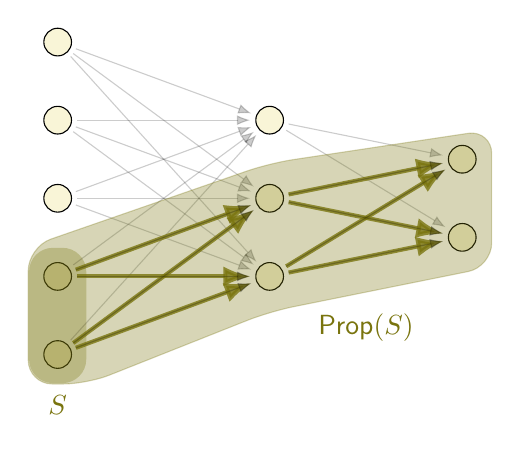
\begin{tikzpicture}[loose/.style={inner sep=.7em},edge/.style = {->,-Latex},
    oval/.style={ellipse,draw}]

    %--------------------------------------------
    % Nodes
    \node[circle,minimum size=10pt,inner sep=0pt,outer sep=2pt,fill=gruvwhite,draw](a){};
    
    \node[below=0.5 of a,circle,minimum size=10pt,inner sep=0pt,outer sep=2pt,fill=gruvwhite,draw](b){};
    
    \node[below=0.5 of b,circle,minimum size=10pt,inner sep=0pt,outer sep=2pt,fill=gruvwhite,draw](c){};
    
    \node[below=0.5 of c,circle,minimum size=10pt,inner sep=0pt,outer sep=2pt,fill=gruvwhite,draw](d){};
    
    \node[below=0.5 of d,circle,minimum size=10pt,inner sep=0pt,outer sep=2pt,fill=gruvwhite,draw](e){};
    
    \node[right=2.2 of b,circle,minimum size=10pt,inner sep=0pt,outer sep=2pt,fill=gruvwhite,draw](f){};
    
    \node[right=2.2 of c,circle,minimum size=10pt,inner sep=0pt,outer sep=2pt,fill=gruvwhite,draw](g){};
    
    \node[right=2.2 of d,circle,minimum size=10pt,inner sep=0pt,outer sep=2pt,fill=gruvwhite,draw](h){};
    
    \node[right=2.2 of $(f)!0.5!(g)$,circle,minimum size=10pt,inner sep=0pt,outer sep=2pt,fill=gruvwhite,draw](i){};

    \node[right=2.2 of $(g)!0.5!(h)$,circle,minimum size=10pt,inner sep=0pt,outer sep=2pt,fill=gruvwhite,draw](j){};
    
    %--------------------------------------------
    % The set S
    \node[fill=gruvgreen, color=gruvgreen, very thick, opacity=0.3,rectangle,rounded corners=2ex,fit=(d) (e)]{};

    \node [color=gruvgreen,opacity=1,below=0.4 of $(e)$]{$S$};
    
    %--------------------------------------------
    % Edges
    % How to color an edge:
    % \draw[edge, line width=1.5pt, color=gruvgreen, opacity=0.8] (a) to (g);
    \draw[edge, color=black, opacity=0.2] (a) -- (f) node [near start, above] {};
    \draw[edge, color=black, opacity=0.2] (a) -- (g) node [near start, above] {};
    \draw[edge, color=black, opacity=0.2] (a) -- (h) node [near start, above] {};
    
    \draw[edge, color=black, opacity=0.2] (b) -- (f) node [near start, above] {};
    \draw[edge, color=black, opacity=0.2] (b) -- (g) node [near start, above] {};
    \draw[edge, color=black, opacity=0.2] (b) -- (h) node [near start, above] {};

    \draw[edge, color=black, opacity=0.2] (c) -- (f) node [near start, above] {};
    \draw[edge, color=black, opacity=0.2] (c) -- (g) node [near start, above] {};
    \draw[edge, color=black, opacity=0.2] (c) -- (h) node [near start, above] {};

    \draw[edge, color=black, opacity=0.2] (d) -- (f) node [near start, above] {};
    
    % ALTERNATE THESE
    \draw[edge, color=black, opacity=0.2] (d) -- (g) node [near start, above] {};
    \draw[edge, color=black, opacity=0.2] (d) -- (h) node [near start, above] {};

    \draw[edge, color=black, opacity=0.2] (e) -- (f) node [near start, above] {};

    % ALTERNATE THESE
    \draw[edge, color=black, opacity=0.2] (e) -- (g) node [near start, above] {};
    \draw[edge, color=black, opacity=0.2] (e) -- (h) node [near start, above] {};
    
    \draw[edge, color=black, opacity=0.2] (f) -- (i) node [near start, above] {};
    
    % ALTERNATE THESE
    \draw[edge, color=black, opacity=0.2] (g) -- (i) node [near start, above] {};
    \draw[edge, color=black, opacity=0.2] (h) -- (i) node [near start, above] {};

    \draw[edge, color=black, opacity=0.2] (f) -- (j) node [near start, above] {};
    
    % ALTERNATE THESE
    \draw[edge, color=black, opacity=0.2] (g) -- (j) node [near start, above] {};
    \draw[edge, color=black, opacity=0.2] (h) -- (j) node [near start, above] {};


    \draw[edge, line width=1.5pt, color=gruvgreen, opacity=0.8] (d) to (g);
    \draw[edge, line width=1.5pt, color=gruvgreen, opacity=0.8] (d) to (h);
    \draw[edge, line width=1.5pt, color=gruvgreen, opacity=0.8] (e) to (g);
    \draw[edge, line width=1.5pt, color=gruvgreen, opacity=0.8] (e) to (h);
    \draw[edge, line width=1.5pt, color=gruvgreen, opacity=0.8] (g) to (i);
    \draw[edge, line width=1.5pt, color=gruvgreen, opacity=0.8] (h) to (i);
    \draw[edge, line width=1.5pt, color=gruvgreen, opacity=0.8] (g) to (j);
    \draw[edge, line width=1.5pt, color=gruvgreen, opacity=0.8] (h) to (j);

    %------------------------------------------------------------
    % FRAME 2
    % The propagation of S
    \pause
    \draw[fill=gruvgreen, color=gruvgreen, opacity=0.3, rounded corners=2ex] 
        ([xshift=-0.2cm,yshift=0.2cm] d.north west)
        -- ([yshift=0.2cm] g.north)
        -- ([xshift=0.2cm, yshift=0.2cm] i.north east)
        
        -- ([xshift=0.2cm,yshift=-0.2cm] j.south east)
        -- ([yshift=-0.2cm] h.south)
        -- ([xshift=0.2cm,yshift=-0.2cm] e.south east)
        -- ([xshift=-0.2cm,yshift=-0.2cm] e.south west)
        -- cycle;
    
    \node [color=gruvgreen,opacity=1, below=0.6 of $(h)!0.5!(j)$]{$\Prop(S)$};

    %------------------------------------------------------------
    % FRAME 3
    \pause
    \draw[edge, color=black, opacity=0.2] (d) -- (g) node [near start, above] {};
    \draw[edge, color=black, opacity=0.2] (d) -- (h) node [near start, above] {};
    \draw[edge, color=black, opacity=0.2] (e) -- (g) node [near start, above] {};
    \draw[edge, color=black, opacity=0.2] (e) -- (h) node [near start, above] {};
    \draw[edge, color=black, opacity=0.2] (g) -- (i) node [near start, above] {};
    \draw[edge, color=black, opacity=0.2] (h) -- (i) node [near start, above] {};
    \draw[edge, color=black, opacity=0.2] (g) -- (j) node [near start, above] {};
    \draw[edge, color=black, opacity=0.2] (h) -- (j) node [near start, above] {};
\end{tikzpicture}

\end{document}